\begin{frame}[parent={cmap:software-testing-foundations}, hasprev=false, hasnext=true]
\frametitle{Test criterion}

\begin{block:fact}{Test techniques and criteria}
\begin{itemize}
	\item Test techniques provides a grounded theory on how we should test our
	software:
	\begin{itemize}
		\item What are the sources of test requirements?

		\item What features of the sources should be exploited?
	\end{itemize}

	\item However, in order to successfully test a software, it must be
	throughly specified how the techniques should be applied.
	\begin{itemize}
		\item Any by successfully we mean: to find errors.
	\end{itemize}
\end{itemize}
\end{block:fact}


\begin{block:fact}{How to increase efficacy}
\begin{itemize}
	\item Test requirements should be established so they explore not only
	what the software should do, but also what it should \textbf{not} do.

	\item A measure should also be provided, so that a stop criteria can be
	defined for the test activity.
\end{itemize}
\end{block:fact}
\end{frame}



\begin{frame}[hasprev=true, hasnext=true]
\label{concept:test-criterion}
\frametitle{Test criterion}

\begin{block:concept}{Definition}
A test criterion systematizes the way test requirements are
generated from the source of information (specification, source code,
historical fault database, etc.).
\end{block:concept}

\begin{block:fact}{}
\begin{itemize}
	\item A test criterion provides a systematic way to select test cases.
	\begin{itemize}
		\item A test criterion divides the input domain.
	\end{itemize}

	\item When no faults are found, test criterion provides an indication of
	how test cases should be selected in order to establish a high level of
	confidence of product correction.
\end{itemize}
\end{block:fact}


\hfill
\refie{example:test-criterion}{\beamerbutton{Example: Test criterion example}}
\end{frame}


\begin{frame}
\frametitle{Test criterion}

\begin{block:fact}{Test criterion attributes}
\begin{itemize}
	\item A test criterion can be compared based on cost, efficacy and
	strength.
\end{itemize}
\end{block:fact}

\begin{block:fact}{}
    \centering
    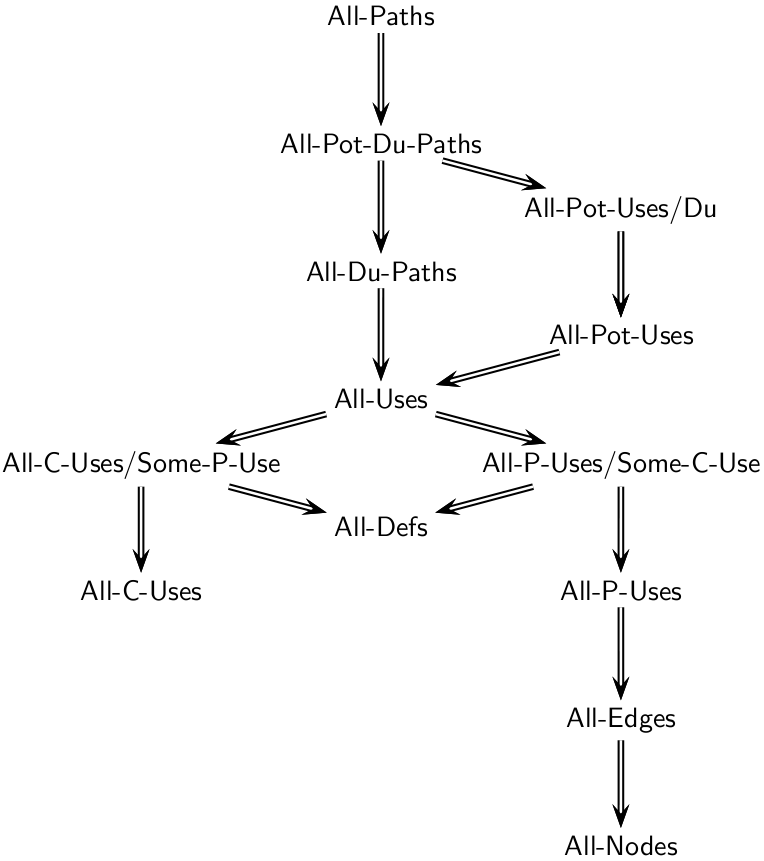
\includegraphics[width=4cm]{subsume-relation}
\end{block:fact}
\end{frame}


\begin{frame}[hasprev=true, hasnext=false]
\frametitle{Test criterion}

\begin{block:fact}{Test coverage}
\begin{itemize}
	\item A test criteria can be used either to evaluate the program under
	testing or to evaluation the thoroughness of the test set.
\end{itemize}
\end{block:fact}

\begin{block:concept}{Test selection criterion}
The test criterion is used to select test cases to evaluate the program under
testing.
\end{block:concept}


\begin{block:concept}{Test evaluation criterion}
The test criterion is used to evaluate the test sets.
\end{block:concept}
\end{frame}


% Test cases representing unexpected and invalid input conditions seem to
% have a higher error-detection yield than do test cases for valid input
% conditions~\cite[p. 18]{myers:2004}.
% \begin{itemize}
%	\item Programs must be examined for unwanted side effects~\cite[p. 18]{myers:2004}.
% \end{itemize}

